% Copyright 2024 Kieran W Harvie. All rights reserved.

\section{Barycentric Coordinates}
Let $P_k$ be the points of an $n$-simplex.
Then for any point $Q$ in the interior there exists a unique set of scalars $\lambda_k$ such that:
\begin{equation*}
\begin{aligned}
	0\leq&\lambda_k\\
	1=&\sum_{k=1}^n\lambda_n\\
	Q=&\sum_{k=1}^nP_n\lambda_n\\
\end{aligned}
\end{equation*}
These scalars are called the barycentric coordinates of the point $Q$.
In this section I will review the $n=2$ case, where the $n$-simplexes are triangles.

\subsection{Etymology}	
This is something that may be obvious to everyone but went over my head for a while.
The `bary' in barycentric isn't from someone named Bary,
but instead comes from the ancient Greek word `barús' meaning heavy,
similar to baryon.

\subsection{Triangles}
Given three 2D points $P_n$ why would we expect the set:
\[\{\lambda_1P_1+\lambda_2P_2+\lambda_3P_3|\lambda_1+\lambda_2+\lambda_3 = 1,\,\lambda_1 \geq 0,\,\lambda_2 \geq 0,\,\lambda_3 \geq 0\}\]
To have anything to do with triangles?
Well consider the function $f:\mathbb{R}^3\rightarrow\mathbb{R}^2$:
\[f(x,y,z) = P_1x+P_2y+P_3z\]
And consider the subset of $S\subset\mathbb{R}^3$ such that $x,y,z\geq0$ and $x+y+z=1$.
\\

$S$ is an equilateral triangle spanning the points $(1,0,0),\,(0,1,0)$ and $(0,0,1)$,
with the image of these points being the points $P_n$.
And $S$ is defined analogously the span of the barycentric coordinates,
so it's a good starting place to get some intuition.

\subsubsection{$f$ is linear}
This function is clearly linear:
\begin{equation*}
\begin{aligned}
	&f(ax_0+bx_1,ay_0+by_1,az_0+bz_1)\\
	=&P_1(ax_0+bx_1) + P_2(ay_0+by_1)+P_3(az_0+bz_1)\\
	=&a(P_1x_0+P_2y_0+P_3z_0) + b(P_1x_1+P_2y_1+P_3z_1)\\
	=&af(x_1,y_1,z_1)+bf(x_1,y_1,z_1)\\
\end{aligned}
\end{equation*}

\subsubsection{$f$ sends line segments to line segments}
Being linear means it sends line segments to lines segments (Or to a single point point if $f(A)=f(B)$):
\[f(At+B(1-t)) = f(A)t+f(B)(1-t)\] 
The function also keeps the `progress' along the line segment.
The point $Q=At+B(1-t)$ is $t$\% along the line $BA$ and $f(Q)$ is $t$\% along $f(B)f(A)$.

\subsubsection{$f$ is a bounded operator}
From the Cauchy-Schwartz inequality we can see that $f$ is a bounded operator:
\begin{equation*}
\begin{aligned}
	||f(\lambda_1,\lambda_2,\lambda_3)||
	=&(\lambda_1x_1+\lambda_2x_2+\lambda_3x_3)^2+(\lambda_1y_1+\lambda_2y_2+\lambda_3y_3)^2\\
	\leq&(\lambda_1^2+\lambda_2^2+\lambda_3^2)(x_1^2+x_2^2+x_3^2)+(\lambda_1^2+\lambda_2^2+\lambda_3^2)(y_1^2+y_2^2+y_3^2)\\
	=&(\lambda_1^2+\lambda_2^2+\lambda_3^2)(x_1^2+x_2^2+x_3^2+y_1^2+y_2^2+y_3^2)\\
\end{aligned}
\end{equation*}
For $(\lambda_1,\lambda_2,\lambda_3)\in S$ we have:
\[\lambda_1^2+\lambda_2^2+\lambda_3^2 \leq 1\]
meaning:
\[s\in S \Rightarrow ||f(s)|| \leq x_1^2+x_2^2+x_3^2+y_1^2+y_2^2+y_3^2\]
Hence all geometry in the image of $S$ takes place is a fixed circle around the origin.
While I don't think this result is technically necessary it does put my mind at ease about weird "projective geometry at infinity" edge cases.
\\

Curiously, 
we can make the inequality strict if we assume the triangle is non-degenerate.
Since there's equality in Cauchy-Schwartz iff:
\[k(x_1,x_2,x_3)=(\lambda_1,\lambda_2,\lambda_3)=l(y_1,y_2,y_3)\]
Which contradicts the triangle being non-degenerate.

\subsubsection{Interior}
Let $Q = (\lambda_1,\lambda_2,\lambda_3)\in S$ and $Q' = \frac{1}{\lambda_1+\lambda_2}(\lambda_1,\lambda_2,0)$, we can write:
\begin{equation*}
\begin{aligned}
	Q'=&\frac{\lambda_1}{\lambda_1+\lambda_2}(1,0,0)+\left(1-\frac{\lambda_1}{\lambda_1+\lambda_2}\right)(0,1,0)\\
	Q =& (1-\lambda_3)Q'+\lambda_3(0,0,1)\\
\end{aligned}
\end{equation*}
Which shows $Q'$ as being on the line segment $P_1P_2$ and $Q$ on $Q'P_3$:
\begin{center}
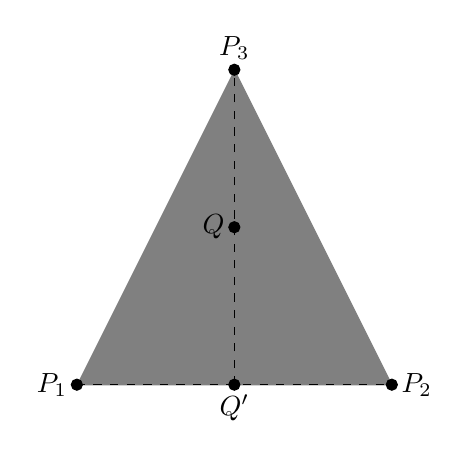
\begin{tikzpicture}[every node/.style={black}]
	\coordinate (P1) at (-2,0);
	\coordinate (P2) at (2,0);
	\coordinate (P3) at (0,4);

	\coordinate (Q') at (0,0);
	\coordinate (Q) at (0,2);

	\filldraw[gray] (P1) -- (P2) -- (P3);

	\draw[dashed] (P1) -- (P2);
	\draw[dashed] (Q') -- (P3);


	\filldraw (Q) node[left] {$Q$} circle (2pt);
	\filldraw (Q') node[below] {$Q'$} circle (2pt);
	\filldraw (P1) node[left] {$P_1$} circle (2pt);
	\filldraw (P2) node[right] {$P_2$} circle (2pt);
	\filldraw (P3) node[above] {$P_3$} circle (2pt);
\end{tikzpicture}
\end{center}
Because $Q'$ is on $P_1P_2$,
the opposite side to $P_3$,
$Q$ is on the segment between a point $P_3$ and that points opposite side $P_1P_2$ and hence is an interior point of $P_1P_2P_3$.
Hence $S\subset P_1P_2P_3$, 
this argument can be reversed to show that $P_1P_2P_3 \subset S$ and thus equality.
\\

Because of how $f$ preserves line segments,
the same stands for $f(Q')$ and $f(Q)$,
The same stands for $f(S) = f(P_1)f(P_2)f(P_3)$.

\subsection{Area coordinates}
\begin{center}
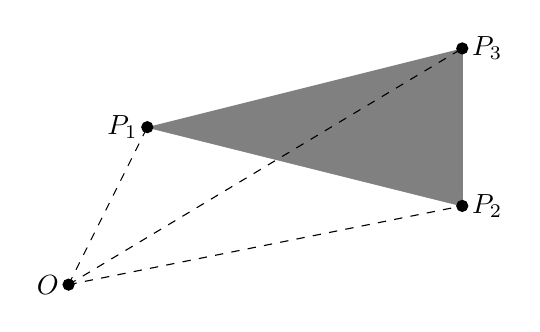
\begin{tikzpicture}[every node/.style={black}]
	\coordinate (O) at (0,0);
	\coordinate (P1) at (1,2);
	\coordinate (P2) at (5,1);
	\coordinate (P3) at (5,3);


	\filldraw[gray] (P1) -- (P2) -- (P3);

	\draw[dashed] (O) -- (P1);
	\draw[dashed] (O) -- (P2);
	\draw[dashed] (O) -- (P3);

	\filldraw (O) node[left] {$O$} circle (2pt);
	\filldraw (P1) node[left] {$P_1$} circle (2pt);
	\filldraw (P2) node[right] {$P_2$} circle (2pt);
	\filldraw (P3) node[right] {$P_3$} circle (2pt);
\end{tikzpicture}
\end{center}
The (unsigned) area of a triangle with points $P_1P_2P_3$ is given by:
\begin{equation*}
\begin{aligned}
	&\frac{1}{2}\left|\begin{vmatrix} x_1&x_2\\y_1&y_2\end{vmatrix} + \begin{vmatrix} x_2&x_3\\y_2&y_3 \end{vmatrix} + \begin{vmatrix} x_3&x_1\\y_3&y_1\end{vmatrix}\right|\\
	=&\frac{1}{2}(x_1(y_3-y_2)+x_2(y_1-y_3)+x_3(y_2-y_1))\\
\end{aligned}
\end{equation*}
This follows directly from the determinant being the signed area of the parallelogram spanned by its column vectors and can be rewritten, to isolate $P_1$, as:
\[\frac{1}{2}\big|x_1(y_3-y_2)-y_1(x_3-x_2)+x_3y_2-x_2y_3\big|\]
Let $Q$ have barycentric coordinates $(\lambda_1,\lambda_2,\lambda_3)$ and consider the area of the triangle $P_2P_3Q$:
\[\frac{1}{2}(\big|\lambda_1x_1+ \lambda_2x_2 + \lambda_3x_3)(y_3-y_2)-(\lambda_1y_1+ \lambda_2y_2 + \lambda_3y_3)(x_3-x_2)+x_3y_2-x_2y_3\big|\]
Considering just the first part shows that the like term, $x_ny_m$ where $n=m$, cancel to give:
\begin{equation*}
\begin{aligned}
	&(\lambda_1x_1+ \lambda_2x_2 + \lambda_3x_3)(y_3-y_2)-(\lambda_1y_1+ \lambda_2y_2 + \lambda_3y_3)(x_3-x_2)\\
	=&\lambda_1(x_1(y_3-y_2)-y_1(x_3-x_2))+ (\lambda_2x_2 + \lambda_3x_3)(y_3-y_2)-(\lambda_2y_2 + \lambda_3y_3)(x_3-x_2)\\
	=&\lambda_1(x_1(y_3-y_2)-y_1(x_3-x_2))+ \lambda_2(x_2y_3-x_3y_2) +\lambda_3(x_2y_3-x_3y_2)\\
	=&\lambda_1(x_1(y_3-y_2)-y_1(x_3-x_2))+ (1-\lambda_1)(x_2y_3-x_3y_2)\\
\end{aligned}
\end{equation*}
And hence and area of the triangle as:
\[\frac{\lambda_1}{2}\big|x_1(y_3-y_2)-y_1(x_3-x_2)+x_3y_2-x_2y_3\big|\]
This is why barycentric coordinates for triangles are also called area coordinates.
Because the first coordinate is the ratio of the area of the total triangle to $P_2P_3Q$,
and likewise for the other coordinates.
\\

\subsection{Some Relations}
Some relations between barycentric coordinates I doodled while waiting for something.
\\
The sum of squares is basically the norm to the center:
\begin{equation*}
\begin{aligned}
	&\left(\lambda_1-\frac{1}{3}\right)^2+\left(\lambda_2-\frac{1}{3}\right)^2+\left(\lambda_3-\frac{1}{3}\right)^2\\
	=&\lambda_1^2+\lambda_2^2+\lambda_3^2-\frac{2}{3}(\lambda_1+\lambda_2+\lambda_3)+\frac{1}{3}\\
	=&\lambda_1^2+\lambda_2^2+\lambda_3^2+\frac{1}{3}\\
\end{aligned}
\end{equation*}
And the second symmetric sum is basically the negative of the norm to the center:
\begin{equation*}
\begin{aligned}
	&\lambda_1\lambda_2+\lambda_2\lambda_3+\lambda_1\lambda_3\\
	=& \frac{1}{2}\bigg((\lambda_1+\lambda_2+\lambda_3)^2 -(\lambda_1^2+\lambda_2^2+\lambda_3^2)\bigg)\\
	=& \frac{1}{2}\bigg(1 -(\lambda_1^2+\lambda_2^2+\lambda_3^2)\bigg)\\
\end{aligned}
\end{equation*}
From the Sedrakyan's inequality we have a lower bound on the interpolation of the reciprocals of positive numbers $a,b,$ and $c$:
\begin{equation*}
\begin{aligned}
	\frac{1}{a+b+c} =& \frac{(\lambda_1+\lambda_2+\lambda_3)^2}{a+b+c} \\
	\leq& \frac{\lambda_1^2}{a}+\frac{\lambda_2^2}{b}+\frac{\lambda_3^2}{c}\\
	\leq& \frac{\lambda_1}{a}+\frac{\lambda_2}{b}+\frac{\lambda_3}{c}\\
\end{aligned}
\end{equation*}
Changing variable use in the same inequality gives:
\[(x+y+z)^2 = \frac{(x+y+z)^2}{\lambda_1+\lambda_2+\lambda_3} \leq \frac{x^2}{\lambda_1} +\frac{y^2}{\lambda_2} +\frac{z^2}{\lambda_3}\]
Which is interpolation of squares,
but over reciprocals of the barycentric coordinates.
\\
Consider the function:
\[f(\lambda_1,\lambda_2,\lambda_3) = \lambda_1\lambda_2(1-\lambda_3)+\lambda_1\lambda_3(1-\lambda_2)+\lambda_2\lambda_3(1-\lambda_1)\]
Interestingly this function is $0$ at the triangle vertices but on the edges, WLOG the edge opposite $P_1$, we get a parabola:
\[f(0,t,1-t) = t(1-t)\]
Looking at the gradient of the function,
recalling that it is a function in the 3D space,
we get:
\[\nabla f = (-\lambda_2\lambda_3,-\lambda_1\lambda_3,-\lambda_1\lambda_2)\]
It always points to the origin and in symmetric around the line from the origin to the center of the triangle.
Hence the center is the maximum and it decreases with radial symmetry.
This radial symmetry is squished by the transform to 2D space,
but can still be used as a displacement to make a triangle wax/wane while keeping the corner the same.

\subsection{Affine Transformations}
While working on something else I was reminded of the formula for the barycentric coordinates in $3$ dimensions,
easily generalized to other dimensions,
is:
\[
\begin{bmatrix}
	x_0&x_1&x_2&x_3\\
	y_0&y_1&y_2&y_3\\
	z_0&z_1&z_2&z_3\\
	1&1&1&1\\
\end{bmatrix}
\begin{bmatrix}
	\lambda_0\\\lambda_1\\\lambda_2\\\lambda_3\\
\end{bmatrix}
=
\begin{bmatrix}
	x\\y\\z\\1\\
\end{bmatrix}
\]
And I noticed the right hand side is a homogeneous vector,
has a final element of $1$.
It is a standard tick to combine a $n\times n$ matrix $M$ an $n$ dimensional vectors $v$ and $u$ into:
\[\begin{bmatrix}
	M&v\\
	0&1\\
\end{bmatrix}
\begin{bmatrix}
	u\\1\\
\end{bmatrix}
=
\begin{bmatrix}
	Mu+v\\1\\
\end{bmatrix}
\]
Such matrices are called homogeneous matrices and they take homogeneous vector to homogeneous vectors,
they also the same this as affine transformations!
Meaning it directly and cleanly follows from multiplying both sides by some homogeneous matrix that barycentric coordinates are invariant under affine transformations:
\[\begin{aligned}
\begin{bmatrix}
	P_0&P_1&P_2&P_3\\
	1&1&1&1\\
\end{bmatrix}
\begin{bmatrix}
	\lambda_0\\\lambda_1\\\lambda_2\\\lambda_3\\
\end{bmatrix}
	=&
\begin{bmatrix}
	P\\1\\
\end{bmatrix}
\\
\Rightarrow
\begin{bmatrix}
	MP_0+T&MP_1+T&MP_2+T&MP_3+T\\
	1&1&1&1\\
\end{bmatrix}
\begin{bmatrix}
	\lambda_0\\\lambda_1\\\lambda_2\\\lambda_3\\
\end{bmatrix}
	=&
\begin{bmatrix}
	MP+T\\1\\
\end{bmatrix}
\end{aligned}\]


% Trilinear conversion?

%The altitude of $P_1$ is perpendicular to $\overline{P_2P_3}$ giving it a gradient of:
%\[-\left(\frac{y_3-y_2}{x_3-x_2}\right)^{-1}= \frac{x_2-x_3}{y_3-y_2}\]
%Hence the foot lies at the intersection of:
%\begin{equation*}
%\begin{aligned}
%	0=&(y_3-y_2)(x-x_2)-(x_3-x_2)(y-y_2)\\
%	0=&(x_3-x_2)(x-x_1)+(y_3-y_2)(y-y_1)\\
%\end{aligned}
%\end{equation*}
%Giving the cool relations:
%\begin{equation*}
%\begin{aligned}
%	0=&(y_3-y_2)^2(x-x_2)+(x_3-x_2)^2(x-x_1)+(x_3-x_2)(y_3-y_2)(y_2-y_1)\\
%	0=&(x_3-x_2)^2(y-y_2)-(y_3-y_2)^2(y-y_1)+(x_3-x_2)(y_3-y_2)(x_2-x_1)\\
%\end{aligned}
%\end{equation*}
%
